\chapter{Contribution} % possible chapter for Projects
\label{chap:contribution}
%----------------------------------------------------------------------------------------
\section{Introduction to the Fair-by-Design Workflow}
The following chapter unveils the core of the research—an innovative Fair-by-Design workflow meticulously crafted to address the pressing issue of bias mitigation within AI systems. It is important to note that, among all the techniques presented in the "State of the Art" chapter, this workflow primarily focuses on the concepts of pre-processing techniques for bias mitigation. 

The Fair-by-Design concept underlines the commitment to infusing fairness principles into the very fabric of AI development. It signifies the endeavor to create AI systems that are not only technologically proficient but also ethically responsible. 

The Fair-by-Design workflow serves as the linchpin of this research. It guides the approach to designing and developing AI systems that are inherently fair, impartial, and equitable. The challenge of bias mitigation cannot be relegated to a mere post hoc consideration; it must be foundational. By introducing fairness considerations at the outset of the AI system design, the aim is to rectify biases before they become ingrained in decision-making processes. 

In the pages that follow, the intricacies of this workflow will be explored, providing a step-by-step elucidation of its various components and how they collectively contribute to the realization of a fair and unbiased AI system. This workflow will not only be a central theme throughout this chapter but also a thread that ties the entire thesis together. It signifies the commitment to addressing bias and promoting fairness within AI systems, particularly in the context of the educational domain. 

The journey will embark on a comprehensive exploration of the Fair-by-Design workflow, with the ultimate goal of mitigating bias, ensuring fairness, and achieving equitable outcomes in AI-driven decision-making.

\section{Workflow description}
The workflow presented in this work is composed of 5 different steps:

\subsection{Data acquisition}
The data acquisition stage represents the critical initial phase responsible for sourcing and gathering the data that will serve as the lifeblood of the AI system. This foundational step plays an indispensable role in ensuring the subsequent phases of the workflow have access to the data necessary for comprehensive analysis and model development. 

The data acquisition stage involves a series of well-defined processes and methodologies aimed at retrieving, collating, and preparing the data. These processes often commence with the identification of the data sources, including databases, APIs, web scraping, or sensor inputs, among others. The selection of data sources is guided by the specific requirements of the AI system and the nature of the problem at hand. 

Once data sources are identified, the data acquisition stage proceeds with data retrieval and extraction. This phase can encompass techniques like data scraping, data transformation, data cleaning, and data enrichment. The objective is to obtain a high-quality and comprehensive dataset, free from errors or inconsistencies, and ready for analysis. 

Data acquisition is a multifaceted process that may also involve considerations related to data privacy, ethics, and legal compliance. This is especially crucial when handling sensitive or personal information, necessitating strict adherence to data protection regulations and ethical principles. 

In summary, the data acquisition stage serves as the gateway to the entire workflow, providing the foundational data needed for subsequent phases, such as data preprocessing, model development, and validation. Its successful execution is paramount in ensuring the overall success and fairness of the AI system.

\subsection{Data pre-processing}
The data pre-processing stage stands as a pivotal component within the workflow, responsible for executing essential operations on the data that has been acquired in the previous stage. This preparatory phase encompasses a range of transformative activities, each aimed at enhancing the quality, reliability, and suitability of the data for subsequent analysis and modeling. 

The core operations conducted during data pre-processing encompass several critical dimensions. Firstly, the stage addresses the management of missing data, including the filling of null or missing values. This operation is essential to mitigate the potential for information loss and ensure that the dataset remains complete and robust. Various techniques, such as imputation, interpolation, or removal, may be employed to address missing values, guided by the specific dataset and the problem's context. 

Another fundamental aspect of data pre-processing involves data normalization, which serves to standardize the data's scale and distribution. This normalization ensures that different attributes within the dataset are on the same scale, preventing any single attribute from disproportionately influencing the analysis or modeling process. Techniques like Min-Max scaling, z-score normalization, or log transformation are commonly employed to achieve this standardization. 

Furthermore, the data pre-processing stage may involve attribute selection or removal based on a predefined policy. Attributes that are deemed irrelevant, redundant, or not aligned with the objectives of the AI system may be excluded from the dataset. This step not only reduces the dimensionality of the data but also enhances the model's efficiency and interpretability. 

Data pre-processing is a multifaceted and nuanced endeavor that plays a critical role in setting the stage for subsequent phases of the workflow. Its meticulous execution ensures that the data is clean, complete, and appropriately prepared for the modeling and validation processes that follow. 

In summary, the data pre-processing stage serves as a foundational and indispensable link in the workflow chain, working to prepare and refine the data acquired in the previous stage, ultimately contributing to the achievement of fairness and accuracy in the AI system.

\subsection{Fairness pre-processing}
The integration of fairness considerations marks a critical juncture within the workflow, as it is the stage where fairness is addressed, thereby imbuing the entire process with the ethos of "fair-by-design." This phase represents the proactive commitment to fairness, a fundamental principle guiding the development of equitable and unbiased AI systems. 

The presence and nature of this step within the workflow are contingent upon the underlying assumptions regarding fairness. In some instances, when no explicit assumptions about fairness are made, this step may be void, and the workflow proceeds with a more conventional approach. However, for situations where fairness is a paramount concern, this stage becomes instrumental. 

One approach to addressing fairness, particularly in the context of "fairness through unawareness," involves the removal of protected attributes from the dataset. This approach seeks to mitigate the impact of sensitive attributes, such as race, gender, or ethnicity, on the AI model's predictions by excluding these attributes from the analysis. While it offers a degree of fairness, it may not comprehensively address fairness challenges. 

An alternative and more comprehensive approach is to incorporate one of the algorithms proposed in this work, which are presented in the following chapters. These algorithms are specifically designed to tackle fairness challenges and mitigate biases within the AI system. They offer a proactive and targeted means of addressing fairness, going beyond the scope of "fairness through unawareness." 

The inclusion of these algorithms signifies a commitment to fairness that extends from the earliest stages of AI system design. By actively integrating fairness into the workflow, the goal is to ensure that the AI system generates predictions and decisions that are not only accurate but also equitable and just. 

In summary, the fairness integration step represents a pivotal phase in the "fair-by-design" workflow. Its presence and nature are shaped by the assumptions and priorities related to fairness, and it serves as a proactive means of addressing bias and promoting fairness within the AI system.

\subsection{Model Tuning}
The model training step represents a pivotal phase within the workflow, entrusted with the critical responsibility of developing a robust and accurate AI model using the data obtained in the previous stage. This phase is the crucible where data is transformed into actionable insights and predictions. 

The model training process begins with the selection of an appropriate algorithm or model architecture tailored to the specific objectives of the AI system. The chosen model is then fed with the pre-processed data, which has been meticulously cleaned, normalized, and, where applicable, imbued with fairness considerations. 

The model training phase leverages advanced techniques and methodologies to iteratively refine the model's parameters, enhancing its predictive capabilities. This optimization process seeks to achieve the delicate balance of minimizing prediction errors while simultaneously upholding the principles of fairness, equity, and unbiased decision-making. 

The training phase may involve a range of considerations, such as hyperparameter tuning, cross-validation, and regularization, to fine-tune the model's performance. Notably, in the context of "fair-by-design," the model training process may also integrate fairness-aware algorithms or techniques proposed in this work, ensuring that fairness is ingrained within the model's learning process. 

Throughout the model training phase, continuous monitoring and evaluation are crucial to assess the model's performance, including its fairness outcomes. Metrics and criteria related to fairness, accuracy, and ethical considerations are employed to gauge the model's effectiveness in producing equitable and unbiased predictions. 

The culmination of the model training phase results in a well-honed AI model, capable of making informed, accurate, and fair predictions. It is the embodiment of the data's transformation into actionable knowledge, and it is primed to contribute to the overarching goals of the AI system. 

In summary, the model training step is central to the workflow, where data is transmuted into the intelligence and predictive power of the AI system. It embodies the principles of fairness, accuracy, and ethical decision-making, shaping the AI model into a powerful tool for promoting equity and justice.

\subsection{Performance evaluation}
The model validation step represents a pivotal phase within the workflow, focused on the rigorous evaluation of the AI model previously trained. This evaluation process is essential for ensuring the model's performance, fairness, and overall effectiveness. 

Model validation begins with the development of comprehensive evaluation criteria and metrics. These criteria encompass a range of dimensions, including predictive accuracy, robustness, and ethical considerations related to fairness. Accuracy metrics assess the model's ability to make correct predictions, while fairness metrics gauge its performance in generating equitable and unbiased outcomes. 

To assess predictive accuracy, common metrics such as precision, recall, F1 score, and area under the receiver operating characteristic curve (AUC-ROC) may be employed. These metrics provide a quantitative measure of the model's predictive power and its ability to discriminate between different classes or categories. 

In the context of fairness, specialized fairness metrics, including disparate impact, equal opportunity, and demographic parity, are utilized to evaluate the model's performance with respect to different demographic groups. These metrics offer insights into the model's propensity to generate disparate outcomes based on sensitive attributes like race, gender, or ethnicity. 

The model validation phase also incorporates techniques like cross-validation to assess the model's robustness and generalizability. Cross-validation involves partitioning the data into multiple subsets and evaluating the model's performance on each subset, ensuring that it can make consistent and accurate predictions across different data splits. 

Furthermore, model validation may involve sensitivity analyses, where the model's performance is evaluated under varying conditions or with perturbed data to identify potential vulnerabilities and areas for improvement. 

The results of the model validation are integral to gauging the model's effectiveness, uncovering potential biases, and making informed decisions about further refinement or deployment. The insights gained from the validation process contribute to the ongoing quest for fairness, accuracy, and ethical decision-making within the AI system. 

In summary, the model validation step plays a fundamental role in the workflow, offering a comprehensive evaluation of the AI model's performance, fairness, and predictive power. Its insights are crucial for guiding the system's development and ensuring that it aligns with the principles of fairness, equity, and accuracy. 


Here's the graphical representation of the presented workflow:
\begin{center}
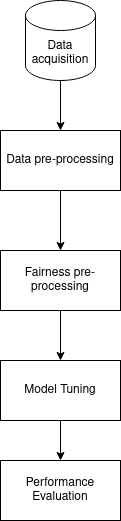
\includegraphics[width=.2\textwidth, height=0.6\textwidth]{FbD.png}
\end{center}
\newpage
In the following are presented the several algorithms that have been put into the \textbf{Fairness pre-processing} step to perform a final comparaison.
\section{Fairness through unawareness with proxy detection}
The algorithm presented in this section is rooted in the fundamental concept of "Fairness through Unawareness." This approach is underpinned by the overarching goal of mitigating bias by removing certain attributes from the dataset. Notably, in this scenario, the removal extends beyond solely the protected attributes, introducing a novel perspective on addressing bias. 

In the spirit of "Fairness through Unawareness," this approach advocates the removal of both the protected attributes and a set of proxy variables. These proxy variables serve as a distinctive feature of the algorithm, as they are strategically identified and eliminated alongside the protected attributes. The proxy variables are defined with a specific focus on aspects that could potentially introduce or perpetuate bias within the AI system. \cite{Gupta2018ProxyF}

The identification and removal of these proxy variables align with the commitment to promoting fairness and equity. By addressing not only the protected attributes but also the factors that may indirectly influence bias, this algorithm adopts a comprehensive approach to bias mitigation. 

The incorporation of proxy variables represents an innovative and proactive step within the workflow, enhancing the system's ability to address bias from multiple angles. This multifaceted approach contributes to the overarching mission of developing AI systems that are not only accurate but also equitable, just, and fair.

\subsection{Algorithm description}
In the following there is the description of the algorithm presented here in its two different versions: the one that comes out using the \textbf{apriori} algorithm and the one that comes out using \textbf{variables only} to perform proxy detection. 


Let's consider a dataset \( D \) belonging to \( \mathbb{R}^{n \times m} \) with \( k \) protected variables. 


\textit{fairness\_evaluation} is defined as follows:
\[
\text{fairness\_evaluation}(v_i, Y) = \lambda(v_i, Y) \quad \forall i \in [1, k]
\]

where:
\begin{align*}
v\_i & : \text{ith attribute belonging to the protected variables}, Y & : \text{output column}.
\end{align*}

The fairness function \( \lambda \) evaluates the relationship between a protected attribute \( v_i \) and the output \( Y \), producing a value that represents the level of fairness for that protected attribute. 


\textit{dataset\_fair} is defined as follows: a dataset \( D \) is considered fair if for every value \( v \) belonging to \textit{fairness\_evaluation}, the following condition holds:
\[ 0.8  < v < 1.25 \] 


Considering the relevance of proxy detection in this algorithm it's important to move on and define the two approaches to detect these variables. 


\subsubsection{Proxy detection via attributes only}
Let's consider the set \( A \), represented as the set of all variables in the dataset excluding the protected variables, and the set \( B \), representing the protected variables.

\textit{proxy\_detection} is defined as follows: for every variable \( \text{var} \) belonging to \( A \) and for every protected variable \( \text{var\_protected} \) belonging to \( B \), the variable is a proxy if the fairness metric \( \lambda(\text{var}, \text{var\_protected}) \) satisfies the condition:

\[
\lambda(\text{var}, \text{var\_protected}) <= 0.8 \quad \text{or} \quad \lambda(\text{var}, \text{var\_protected}) => 1.25
\]

In other words, a variable \( \text{var} \) is considered a proxy if the fairness measure \( \lambda \) between \( \text{var} \) and a protected variable \( \text{var\_protected} \) falls outside the acceptable range ]0.8, 1.25[. 


\subsubsection{Proxy detection via apriori}
It's important to give a brief background of the Association Rule Mining, the family algorithm \textbf{apriori} belongs to.

\begin{enumerate}
    \item \textbf{Association rule mining}:
    Association rule mining represents a pivotal data mining technique employed to unearth intriguing relationships and patterns hidden within extensive datasets. This technique is specifically tailored to the task of identifying associations and correlations among diverse elements present in the data, thereby revealing valuable insights and connections that might otherwise remain concealed. 

    The primary objective of association rule mining is to expose the inherent dependencies between data items or attributes. It scrutinizes the dataset in search of rules that reveal the co-occurrence and relationships between different items. These rules often manifest in the form of "if-then" statements, where the presence of one item is associated with the presence or absence of another. 

    This technique is particularly advantageous when applied to large volumes of data, as it excels in discovering subtle, non-obvious associations that might elude simple statistical analysis. Association rule mining is a versatile tool with a wide array of applications, spanning domains such as market basket analysis, recommendation systems, and fraud detection. 

    The process of association rule mining involves the generation of itemsets and the identification of frequent itemsets—combinations of items that appear together frequently. The algorithm then extracts association rules from these frequent itemsets, offering valuable insights into the relationships and co-occurrences within the data. 

    The outcomes of association rule mining have the potential to drive informed decision-making, such as product recommendations based on customer purchase history, optimizing supply chain management, and identifying suspicious patterns in financial transactions.
    

    \item \textbf{Apriori algorithm}: Suppose to have a set of transactions $T$, each containing a set of items. Let's define:

\begin{itemize}
  \item $I$: the set of all distinct items in the data.
  \item $D$: the set of transactions, each represented by a set of items.
  \item $F_k$: the set of frequent itemsets of length $k$.
\end{itemize}

The Apriori algorithm operates in iterations, generating $F_k$ from $F_{k-1}$.

\textbf{Step 1:} Initialization:
$$F_1 = \{ \text{frequent item } i, i \in I \}$$

\textbf{Step 2:} Candidate itemset generation:
$$C_k = \{ \text{set } c \text{ of items such that } c \subseteq F_{k-1} \}$$

\textbf{Step 3:} Database scan:
$$\text{For each transaction } t \text{ in } D, \text{ increment the support count of each candidate in } C_k \text{ contained in } t.$$

\textbf{Step 4:} Selection of frequent itemsets:
$$F_k = \{ c \in C_k \text{ such that the support of } c \geq \text{ specified threshold} \}$$

\item \textbf{Row Selection with a Confidence Level}: 
suppose to have obtained association rules using the Apriori algorithm. Each rule $R$ is in the form $A \rightarrow B$, where $A$ is the antecedent and $B$ is the consequent. The confidence of $R$ is defined as:

\[
\text{Confidence}(R) = \frac{\text{Support}(A \cup B)}{\text{Support}(A)}
\]

To select rows with a certain confidence level, is considered a confidence threshold $C_{\text{min}}$. If the confidence of a rule $R$ exceeds this threshold, the rule is accepted.

Formally, a rule $A \rightarrow B$ is accepted if:

\[
\text{Confidence}(A \rightarrow B) \geq C_{\text{min}}
\]
In our scenario
\[
C_{\text{min}}
\]
is equal to 0.8. 


The consequent filtering process involves evaluating each rule to ensure it meets this criteria. If the consequent of a rule does not contain any sensitive attributes, that rule is discarded from the final selection. 


Formally, a rule $A \rightarrow B$ is considered if:

\[
\exists b \in B : b \in S
\]

If this condition is not met, the rule is discarded from the final selection.
\end{enumerate}
After this brief introduction of the concepts used to apply this algorithm is presented the approach to detect proxy variables. 

\textit{proxy\_detection} is defined as follows: for each antecedent \( A_i \) belonging to the antecedent list \( \mathcal{A} \), for each consequent \( C_j \) belonging to the consequent list \( \mathcal{C} \), and for each protected variable \( V_k \) belonging to the protected variable list \( \mathcal{V} \), \( A_i \) is a proxy if the fairness metric \( \lambda(A_i, C_j) \) is such that:

\[\lambda(A_i, C_j) <= 0.8 \quad \text{or} \quad \lambda(A_i, C_j) >= 1.25\]

In other words, an antecedent \( A_i \) is considered a proxy if the fairness measure \( \lambda \) between \( A_i \) and a consequent \( C_j \) is outside the acceptable range ]0.8, 1.25[.




There are two other fucnctions that needs to be defined in order to complete our algorithm.




Considering the dataset \( D \) belonging to \( \mathbb{R}^{n \times m} \) and \( k \) as the number of identified proxy variables, the function \( \text{proxy\_free\_dataset} \) is defined as follows:

\[
\text{\textbf{proxy\_free\_dataset}}: D \times \mathbb{R}^{k \times 1} \rightarrow \mathbb{R}^{n \times (m - k)}
\]

where \( j = m - k \) and \( \text{proxy\_free\_dataset}(D) \) yields a dataset \( \mathbb{R}^{n \times j} \) devoid of the proxy variables, ensuring the removal of any potential indirect indicators that may influence sensitive attributes. 



Considering the dataset \( D \) belonging to \( \mathbb{R}^{n \times j} \) where j are the columns obtained after the proxy removals and \( k \) as the number of identified protected variables, the function \( \text{protected\_attributes\_free\_dataset} \) is defined as follows:

\[
\text{\textbf{protected\_attributes\_free\_dataset}}: D \times \mathbb{R}^{k \times 1} \rightarrow \mathbb{R}^{n \times (j - k)}
\]

where \( p = j - k \) and \( \text{protected\_attributes\_free\_dataset}(D) \) yields a dataset \( \mathbb{R}^{n \times p} \) devoid of the protected variables, ensuring the removal of any potential indirect indicators that may influence sensitive attributes.

\subsection{Pseudocode}
Here's the pseudocode of the \emph{Fairness through unawareness with proxy detection}:

\begin{algorithm}[H]
    \KwData{dataset}
    \KwResult{fair dataset}
    \While{\textbf{not} \textit{dataset\_fair(dataset)} \textbf{or} \textit{protected\_attributes} \textbf{in} \textit{dataset}}{
        proxies = \textit{proxy\_detection(dataset)}\;
        \If{proxies \textbf{is empty}}{
            dataset = \textit{protected\_attributes\_free\_dataset(dataset)}\;
        }
        \Else{
            dataset = \textit{proxy\_free\_dataset(dataset)}\;
        }
    }
    \KwRet{dataset}
\end{algorithm}

\subsubsection{dataset\textunderscore fair pseudocode}
Here's the pseudocode that establish if the dataset is either \emph{Fair} or not

\begin{algorithm}[H]
    \KwData{dataset, protected\_attribute}
    \KwResult{Boolean value indicating fairness}
    \If{\textit{fairness\_evaluation(dataset, protected\_attribute)} \textbf{is empty}}{
        \KwRet{\textbf{True}}\;
    }
    \KwRet{\textbf{False}}
\end{algorithm}

\subsubsection{fairness\textunderscore evaluation pseudocode}
Here's the pseudocode to perform the fairness evaluation, given a specific \emph{fairness metric}

\begin{algorithm}[H]
    \KwData{dataset, output\_column, protected\_attributes}
    \KwResult{List of attributes failing fairness evaluation}
    fairness\_evaluation\_list $\gets$ empty list\;
    output $\gets$ dataset[output\_column]\;
    \For{attribute \textbf{in} protected\_attributes}{
        \If{\textit{metric(attribute, output)} $\leq$ 0.8 \textbf{or} \textit{metric(attribute, output)} $\geq$ 1.25}{
            \textit{fairness\_evaluation\_list.append(attribute)}\;
        }
    }
    \KwRet{fairness\_evaluation\_list}
\end{algorithm}

\subsubsection{protected\textunderscore attributes\textunderscore free\textunderscore dataset pseudocode}
Here's the pseudocode to remove protected attributes from the dataset

\begin{algorithm}[H]
    \KwData{dataset, protected\_attributes}
    \KwResult{Dataset with protected attributes removed}
    \For{attribute \textbf{in} protected\_attributes}{
        \textit{dataset.remove(attribute)}\;
    }
    \KwRet{dataset}
\end{algorithm}

\subsubsection{proxy\textunderscore free\textunderscore dataset pdeudocode}
Here's the pseudocode to remove proxy attributes from the dataset

\begin{algorithm}[H]
    \KwData{dataset, proxy\_list}
    \KwResult{Dataset with proxies removed}
    \For{proxy \textbf{in} proxy\_list}{
        \textit{dataset.remove(proxy)}\;
    }
    \KwRet{dataset}
\end{algorithm}

\subsubsection{proxy\textunderscore detection pseudocode}
Here's the pseudocode of proxy\textunderscore detection function. There are 2 scenarios that are presented here, the one in which the \emph{variables only}  approach is used and the one in which the \emph{apriori} approach is used

\begin{enumerate}
    \item \textbf{Variables only}: 
            
\begin{algorithm}[H]
    \KwData{protected\_attributes\_list, attributes}
    \KwResult{List of proxies}
    proxy\_list $\gets$ empty list\;
    \For{protected\_attribute \textbf{in} protected\_attributes\_list}{
        \For{attribute \textbf{in} attributes \textbf{and not in} protected\_attributes\_list \textbf{and not in} proxy\_list}{
            \If{\textit{metric(attribute, protected\_attribute)} $\leq$ 0.8 \textbf{or} \textit{metric(attribute, protected\_attribute)} $\geq$ 1.25}{
                \textit{proxy\_list.append(attribute)}\;
            }
        }
    }
    \KwRet{proxy\_list}
\end{algorithm}

    \item \textbf{Apriori}:

    \begin{algorithm}[H]
    \KwData{apriori\_dataset}
    \KwResult{List of proxies}
    proxy\_list $\gets$ empty list\;
    \For{consequent \textbf{in} apriori\_dataset}{
        \For{antecedent \textbf{in} apriori\_dataset}{
            \If{\textit{metric(antecedent, consequent)} $\leq$ 0.8 \textbf{or} \textit{metric(antecedent, consequent)} $\geq$ 1.25}{
                \textit{proxy\_list.append(antecedent)}\;
            }
        }
    }
    \KwRet{proxy\_list}
\end{algorithm}
\end{enumerate}
\newpage

\section{Fairness through data rebalancing}

In this approach, the paradigm of bias mitigation takes on a unique and innovative perspective, one that prioritizes data augmentation over attribute removal. Unlike traditional approaches that center on the exclusion of specific attributes, this methodology embraces the concept of data augmentation, introducing a distinctive definition of fairness and equity within the AI system.

The essence of this approach revolves around the augmentation of the dataset by introducing new data instances that offer a more comprehensive and inclusive representation of the underlying population. This expanded dataset is designed to be more diverse, representative, and balanced, transcending the limitations of the original data and fostering a more nuanced understanding of fairness. 

The introduction of augmented data instances leads to a redefined notion of fairness within the AI system. Instead of solely focusing on the absence of biased attributes, fairness is now measured in terms of the dataset's inclusivity and its ability to capture the diversity and nuances present within the population it seeks to serve. 

This approach aligns with the broader philosophy of ensuring that AI systems are equitable, just, and capable of making informed and unbiased decisions. By augmenting the dataset, it strives to bridge the gaps in representation and provide a more equitable playing field for all individuals, regardless of their background or characteristics. 

The process of data augmentation necessitates a careful selection of techniques and methodologies that can introduce new data instances while maintaining the integrity and quality of the dataset. These techniques may encompass oversampling, synthetic data generation, or other data synthesis methods, each tailored to the specific context and objectives of the AI system.

\subsection{A New Definition of Fairness}

In traditional fairness definitions, the focus often revolves around ensuring fair treatment for individual protected attributes, denoted as $A_1, A_2, \ldots, A_k$. While this is undoubtedly crucial, a more comprehensive understanding of fairness calls for an examination of fairness in the context of combinations of protected attributes and the output. A new definition of fairness is proposed, which takes into account the representation of all combinations of $k$ protected attributes and the output, aiming for equitable representation across these combinations.

\subsubsection{Equal Representation of Combinations}

A fair dataset is defined as one in which, for each combination of protected attributes $\{A_1, A_2, \ldots, A_k\}$ and the output $O_j$, the representation is equal and proportional. Mathematically, a dataset is fair if:

\[
\forall i_1, i_2, \ldots, i_k, j: \frac{|D_{i_1, i_2, \ldots, i_k, j}|}{|D|} = \text{constant}
\]

where:
- $D$ is the dataset,
- $|D_{i_1, i_2, \ldots, i_k, j}|$ is the number of samples with the specific combination of protected attributes $A_{i_1}, A_{i_2}, \ldots, A_{i_k}$ and output $O_j$,
- $|D|$ is the total number of samples in the dataset.

This entails that any combination of demographic groups, defined by the protected attributes, and the output should have comparable representation, thereby fostering a balanced and unbiased dataset.

\subsubsection{Promoting Comprehensive Fairness}

By striving for equal representation of combinations of protected attributes, is addressed a fundamental aspect of fairness that transcends individual attributes. This approach provides a more nuanced understanding of fairness by considering the intersections of various demographic groups. It encourages a broader examination of potential biases that may arise when considering multiple attributes simultaneously.

Incorporating this definition of fairness into the dataset rebalancing process enables us to promote a comprehensive notion of fairness, aligning with the principles of equal opportunity and non-discrimination across all combinations of protected attributes. Our subsequent algorithm and experimental evaluation are designed to actualize this definition and demonstrate its effectiveness in achieving a more equitable representation within the dataset.

\subsection{Algorithm description}

Let \( D \) be a dataset \( R^{n \times m} \), where \( n \) is the number of samples and \( m \) is the number of features. Let \( k \) be the number of protected variables represented as \( R^{n \times 1} \), and let there be a single output variable represented as \( R^{n \times 1} \).

A rebalancing function \( \mathcal{R} \) can be formally defined as a mapping:

\[
\mathcal{R}: R^{n \times m} \rightarrow R^{l \times m}
\]

where \( l > m \), and the function \( \mathcal{R} \) transforms the input dataset \( D \) of dimensions \( n \times m \) into an output dataset \( D' \) of dimensions \( l \times m \).



Let \( k \) be the number of binary protected variables in the dataset \( D \), and consider the output variable to be binary as well. The number of possible combinations of these variables is \( 2^{(k+1)} \).

Consider a set \( \text{Combination-frequency} \) with occurrences of all \( 2^{(k+1)} \) combinations within the dataset. For each combination, the number of rows in which that combination appears should be equal to the maximum occurrence among all combinations present in the set \( \text{Combination\textunderscore frequency} \). This maximum value is denoted as \( \text{Max}(\text{Combination-frequency}) \).

Mathematically, the number of rows (\( l \)) the final dataset should have for each combination is given by:

\[
l = \text{Max}(\text{Combination-frequency})
\]



Let \( l \) be the desired number of rows for the final dataset. For each combination of values, is calculated the occurrence count \( \text{occurrence}_i \), where \( i \) ranges from 1 to \( 2^{(k+1)} \), with \( k \) being the number of protected binary variables and considering the output variable as binary.

The total number of rows to be added is given by:

\[
\text{total\_rows\_to\_add} = l - \sum_{i=1}^{2^{(k+1)}} \text{occurrence}_i
\]

For each iteration:
\begin{itemize}
    \item The values of the protected and output variables are set according to the specific combination.
    \item For all other attributes, a random value \( \text{random\_value}_{ij} \) is generated, where \( j \) represents the specific attribute and \( i \) represents the row being added for that attribute. \( \text{random\_value}_{ij} \) is within the minimum and maximum range for attribute \( j \).
\end{itemize}

\subsection{Pseudocode}
\begin{algorithm}[H]
    \SetKwInOut{Input}{Input}
    \SetKwInOut{Output}{Output}

    \Input{combination\_set, combination\_frequency, protected\_attributes, dataset\_attributes}
    \Output{Updated dataset}

    max\_frequency $\gets$ max(combination\_frequency)\;
    \For{index $\gets$ 0 \KwTo len(combination\_set)}{
        combination $\gets$ combination\_set[index]\;
        frequency $\gets$ combination\_frequency[index]\;
        \While{frequency $<$ max\_frequency}{
            new\_row $\gets$ empty\;
            \For{(attr, val) \textbf{in} (combination, protected\_attributes)}{
                new\_row[attr] $\gets$ val\;
            }
            \For{attr \textbf{in} dataset\_attributes \textbf{and not in} protected\_attributes}{
                new\_row[attr] $\gets$ random(min(attr), max(attr))\;
            }
            dataset.add(new\_row)\;
            frequency $+$= 1\;
        }
    }
\end{algorithm}
\newpage
%----------------------------------------------------------------------------------------
%\chapter{Implementation} % possible chapter for Projects
%\label{chap:implementation}
%----------------------------------------------------------------------------------------
\section{Dataset description}
Before delving into the intricate details of the algorithm implementations presented earlier, it is imperative to provide a comprehensive overview of the dataset on which these algorithms have been applied. The chosen dataset for this work is the "ULL dataset," an invaluable resource that underpins the empirical exploration of bias mitigation strategies in the context of the educational system in the Canary Islands. 

The ULL dataset is a rich and expansive repository of information, meticulously compiled to capture various facets of the educational landscape within the Canary Islands. This dataset comprises the comprehensive census of students enrolled over four distinct academic years, offering a multifaceted glimpse into the educational ecosystem. 

The dataset encompasses a diverse array of attributes and data points, encapsulating critical information such as student demographics, academic performance, socioeconomic factors, and other pertinent variables. These attributes collectively provide a holistic perspective on the educational landscape, enabling a nuanced analysis of the factors that influence student outcomes and experiences. 

The temporal dimension of the dataset, spanning four academic years, further enriches the analytical potential. It allows for the investigation of temporal trends, shifts in educational policies, and the evolution of student characteristics over time. This temporal depth is particularly valuable when examining the efficacy of bias mitigation strategies, as it facilitates the assessment of their impact across different academic years. 

The ULL dataset is not merely a repository of numbers and statistics; it is a window into the educational opportunities and challenges faced by students in the Canary Islands. By harnessing the insights gleaned from this dataset, it becomes possible to proactively address biases and promote equity within the educational system, ultimately striving for a more inclusive and just educational landscape.

\subsection{Pre-processing operations on ULL dataset}
A deep analysis of the dataset led us to make a first features selection. More specifically for this work only the \emph{important} and \emph{protected} attributes have been selected.
\subsubsection{Protected attributes choice}
After a proper domain analysis the protected attributes selected to be passed to the algorithms have been a subset of the orginal selected:
\begin{enumerate}
    \item sex
    \item capital island: if the student comes from the capital of the city
    \item public\textunderscore private: if the school is public or private
    \item inmigrant: if the student is either inmigrant or not
    \item inmigrant second gen: if the student is either inmigrand of second gen or not
    \item parent expectation
    \item mothly houseold income
    \item cconomic, social and cultural satus index
\end{enumerate}
\subsubsection{Attributes pre-processing}
The dataset documentation provided the information related to the type of each attribute (e.g. Continuous or Categorical). Starting from this information the variables have been pre-processed as follows.
\begin{itemize}
    \item Each categorical attribute has been replaced with an encoded value
    \item For each protected attribute has been computed the following operation:
    \begin{itemize}
        \item If the protected attirbute is a binary one, assuming that the binary values may not be onlu 0 and 1, then the greatest value has been replaced with 1 and the other one with 0.
        \item If the protected attribute is a categorical one then is performed a search of the most frequent value in the column. Then this value in the column is replaced with 1, otherwise with 0. With this policy is established that the fairness must be guaranteed between the most frequent value and the others.
        \item if the protected attribute is a continuous one then is computed the the theshold resulting from the sum of minimum value and maximum value in the column divided by 2. Every value in the column above this threshold is replaced with 1, otherwise with 0. This means that the fairness must be guaranteed between the students that are above the threshold for a specific attribute and the other ones.
    \end{itemize}
\end{itemize}

\subsection{Goal of this work}
The several output in this dataset are considered as protected attributes. More specifically the goal of this work is to predict the english level of a given student. Since the \emph{level\textunderscore ing} attribute is a categorical ones then the output states if a student has the same level of the majority of the students or if not. The goal is to make the predictor and the prediction fair, this means that the belonging of a student to a specific output, the match indeed, must no be influenced by any other factors rather than the predictor's mechanisms.
\newpage
\section{Fairness through unawareness with proxy detection: implementation}
In this section are reported the several implementative issues and features that have been encountered and designed during the development of this algorithm. Two approaches are explored in detail, the one with \textbf{apriori} and the one in which only the \textbf{variables} have been taken in account. 

\subsection{Proxy detection via apriori}
The implementation of this approach has proceeded according a modular approach and, more specifically, has been developed a module named \emph{fairness} in which there are all the sub-modules needed to implement this approach.
\subsubsection{fairness\textunderscore metric module}
This module has been thought to contain the implementation of the several fairness metrics considered in the context of the study. In our scenario it only contains the implementation of the \emph{Disparate Impact} metric. 

This implementation provides to the user the information about the fairness status of the dataset provided together with the protected attributes, the otuput attribute and the possible values that this value may have: 

\begin{lstlisting}
    def fairness_evaluation(self, dataset: pd.DataFrame, protected_attributes: list, output_column_values: list,
                            output_column: str) -> str:
        """
        This method perform an evaluation of the fairness of a given dataset according to the Disparate Impact metric
        :param dataset: this is the dataset on which to be labelled as fair or unfair
        :param protected_attributes: the list of the protected attributes on which compute the disparate impact value
        :param output_column: the column of the dataset that represents the output
        :return: return 'fair' if the dataset is fair, unfair 'otherwise'
        """
        bias_analysis_dataframe = self.bias_detection(dataset, protected_attributes, output_column_values, output_column)
        return_value = 'unfair'
        for value in bias_analysis_dataframe['Disparate Impact'].values:
            if value <= 0.80 or value >= 1.25:
                return_value = 'unfair'
                break
            else:
                return_value = 'fair'

        return return_value
\end{lstlisting}


\subsubsection{matching module}
This module only contains the method \emph{conscious\textunderscore fairness\textunderscore through\textunderscore unawareness} that can return the dataset in two possible configurations:
\begin{enumerate}
    \item if the dataset is fair it returns the dataset itself only with variables pre-processed. Since these pre-processing operations are performed before the fairness checking these are the same for both scenarios. These operations are the transformation of every \emph{categorical} attribute into a numerical one and the transformation of protected attributes as explained above.
    \item if the dataset is not fair the algorithm looks for the proxies and remove the proxies found if there are some and the protected attributes.
\end{enumerate}
\subsubsection{proxy module}
This module is the core of the whole algorithm. This module contains other two sub-modules. More specifically it contains a module whose goal is to detect proxy and the other one is the module in charge to translate the result of the proxy detection to provide a list of proxies to be used into the \emph{matching} module
\begin{enumerate}
    \item \emph{proxy\textunderscore detection}: this module is the one in which the \emph{apriori} algorithm is applied in order to found the relation between antecedents and consequents with a confidence value of 0.8. The key method of this module is the private method \emph{\textunderscore return\textunderscore apriori\textunderscore dataframe}. This method performs computation on the result of the application of the apriori algorithm. More specifically it returns a dataframe with 3 columns \textbf{Antecedent}, \textbf{Consequent}, \textbf{Confidence} 

    \begin{lstlisting}
        def _return_apriori_dataframe(association_results: list) -> pd.DataFrame:
    """This function returns the dataframe with the association generated by the apriori algorithm

    Args:
        association_results (list): is the list of the association returned by the apriori algorithm

    Returns:
        pd.DataFrame: is the dataframe equivalent to the association result list
    """
    antecedent = []
    consequent = []
    confidence = []

    for association_result in association_results:
        for ordered_statistic in association_result.ordered_statistics:
            antecedent_elements = list(ordered_statistic.items_base)
            antecedent.append(antecedent_elements)
            consequent_elements = list(ordered_statistic.items_add)
            consequent.append(consequent_elements)
            confidence_elements = ordered_statistic.confidence
            confidence.append(confidence_elements)

    antecedent_series = pd.Series(antecedent)
    consequent_series = pd.Series(consequent)
    confidence_series = pd.Series(confidence)

    dataframe = pd.DataFrame(
        {'Antecedent': antecedent_series, 'Consequent': consequent_series, 'Confidence': confidence_series})

    return dataframe
    \end{lstlisting}
    \item \emph{proxy\textunderscore processing}: this module contains two key methods. The first method, \emph{\textunderscore return\textunderscore proxy\textunderscore protected\textunderscore attribute} returns a dataframe in which for each sensitive attribute as consequent are related the antecedents that are the possible proxies for that sensitive attribute. The second method is \emph{proxy\textunderscore fixing}, in which for each antecedent is computed the Disparate impact value related to that consequent with that specific value. Only the variables with DI value lesser than 0.8 or greater than 1.25 are considered as proxies. In the following is reported the code of both methods:
    \begin{lstlisting}
        def _return_proxy_protected_attribute(proxy_variables: pd.DataFrame, protected_attributes: list) -> pd.DataFrame:
    """This method returns a dataframe containing the proxy variables for each sensitive attribute

    Args:
        proxy_variables (pd.DataFrame): the dataframe of the proxy variables (antecedent, consequent, confidence)
        protected_attributes (list): the list of the protected attributes

    Returns:
        pd.DataFrame: _description_
    """
    sensitive_antecedent = []
    sensitive_consequent = []
    for index, proxy_row in proxy_variables.iterrows():
        for consequent in proxy_row['Consequent']:
            for sensitive_attribute in protected_attributes:
                if str(consequent).startswith(sensitive_attribute):
                    sensitive_antecedent.append(proxy_row['Antecedent'])
                    sensitive_consequent.append(consequent)

    dataframe = pd.DataFrame(
        {'Antecedent': pd.Series(sensitive_antecedent), 'Consequent': pd.Series(sensitive_consequent)})

    return dataframe


    \end{lstlisting}
    \begin{lstlisting}
        def proxy_fixing(original_dataset: pd.DataFrame, 
        protected_attributes: list) -> pd.DataFrame:
    """This method returns a dataset with proxy variables founded in the original dataset analyzed.
    In case these proxies lead to unfairness the proxies are deleted

    Args: original_dataset (pd.DataFrame): the dataset on which the proxy variable have to be deleted if they lead to
    unfairness
    protected_attributes (list): the list of protected attribute on which perform the proxy analysis

    Returns:
        pd.DataFrame: returns the dataframe in which the proxies do not lead to fairness
    """
    proxy_variables = return_proxy_variables(original_dataset)
    proxy_variables_for_sensitive_attributes = 
    _return_proxy_protected_attribute(proxy_variables, protected_attributes)
    
    dataset = original_dataset
    for index, row in proxy_variables_for_sensitive_attributes.iterrows():
        for antecedent in row['Antecedent']:
            consequent = row['Consequent']

            disparate_impact_value = _compute_disparate_impact_for_proxy(
                antecedent, consequent,original_dataset)

            if not 0.8 < disparate_impact_value < 1.25 and _proxy_format_to_column(antecedent) not in protected_attributes:
                dataset = _remove_proxy_from_dataset(original_dataset, antecedent)

            else:
                continue

    return dataset

    \end{lstlisting}
\end{enumerate}

\subsection{Proxy detection via variables only: implementation}
The implementation of this approach differs with the implementation of the apriori approach because of the operation of proxy detection and processing have been mixed together and the proxy removal operation has been delegated to the \emph{matching} module. In the following there's the code that computes the proxy detection:
\begin{lstlisting}
    def proxy_detection(dataset: pd.DataFrame, protected_attributes: list, output_column: str) -> list:
    attributes_list = []
    for attr in dataset.columns:
        if attr not in protected_attributes:
            attributes_list.append(attr)
            
          
    if output_column in attributes_list:
        attributes_list.remove(output_column)
        
    proxy_list = []
    for attribute in attributes_list:
        for protected_attribute in protected_attributes:
            if _compute_disparate_impact_for_proxy(attribute, protected_attribute, dataset) == 'PROXY':
                proxy_list.append(attribute)

    return proxy_list

\end{lstlisting}
\newpage
\section{Fairness through data rebalancing: implementation}
The first big difference between this approach and the two previous ones is that no fairness-metrics is used here. The reason behind this is the new definition provided for fairness, where is assumed as a parity in combination occurrance. So the core of this algorithm is the \emph{rebalancing} module in which rows are added to the dataset according to the most frequent combination occurrance in the original dataset.
The key part of this module is the one in which the other attributes are inserted. In this scenario a new value is added considering the minimum and the maximum in the temporary dataset, where this dataset is the dataset in which a certain combination of protected\textunderscore attributes and output is occurred. It's furthermore important to remark that since a value has been  randomically chosen this may alter the distribution for that attribute.
\begin{lstlisting}
    for index in range(0, len(combination_list)):
        combination = combination_list[index]
        temp_dataset = final_dataset.query(return_query_for_dataframe(combination, combination_attributes))
        if combination_frequency[index] == combination_frequency_target:
            continue
        else:
            for counter in range(0, combination_frequency_target - combination_frequency[index]):
                new_row = {}
                for (attr, value) in zip(combination_attributes, combination):
                    new_row[attr] = value
                for attribute in final_dataset.columns:
                    if attribute not in combination_attributes:
                        if is_variable_discrete(temp_dataset, attribute):
                            new_row[attribute] = random.randint(temp_dataset[attribute].min(), temp_dataset[attribute].max())
                        else:
                            new_row[attribute] = random.uniform(temp_dataset[attribute].min(), temp_dataset[attribute].max())
                
                final_dataset.loc[len(final_dataset)] = new_row

\end{lstlisting}